\documentclass[11pt]{book}

%\usepackage{lnote}

\usepackage{CJKutf8,CJKnumb}
%\usepackage{CJKpunct} %a homemade package

\usepackage{fancyhdr}
\usepackage{titlesec}

\usepackage{indentfirst}
\usepackage{paralist}
\usepackage{verbatim}

\usepackage[plain]{fancyref}
\usepackage[bookmarksnumbered,dvipdfmx,unicode, pdfborder=1,breaklinks,colorlinks,linkcolor=RoyalBlue3,urlcolor=blue]{hyperref}
\usepackage{makeidx}

\usepackage{mflogo,texnames}
\usepackage{textcomp}

\usepackage{amsmath,amsfonts,amsthm}

\usepackage[x11names]{xcolor} %must before tikz, x11names defines RoyalBlue3
\usepackage{graphicx}
%\usepackage{ps4pdf} %conflict with tabularx
\usepackage{pstricks,pst-plot,pst-eps}
\usepackage{subfig}
\def\pgfsysdriver{pgfsys-dvipdfmx.def} %put before tikz
\usepackage{tikz}

\usepackage{booktabs,tabularx,multirow,colortbl,longtable}

\usepackage{chapterbib}
\usepackage[sectionbib,super,square,sort&compress]{natbib}


%中文设置
\iffalse
\newcommand{\song}{\CJKfamily{song}}
\newcommand{\fang}{\CJKfamily{ufang}}
\newcommand{\kai}{\CJKfamily{ukai}}
\newcommand{\hei}{\CJKfamily{uhei}}
\fi
%\AtBeginDvi{\special{pdf:tounicode GBK-EUC-UCS2}} %not necessary if use UTF8.

%行距
\renewcommand{\baselinestretch}{1.25}

%页眉页脚
\pagestyle{fancy}
\fancyhf{}
\fancyhead[LE,RO]{\thepage}
\fancyhead[RE]{\leftmark}
\fancyhead[LO]{\rightmark}
\fancypagestyle{plain}{%设置plain页格式
    \fancyhf{}
    \renewcommand{\headrulewidth}{0pt}
}

%章节
\renewcommand{\chaptername}{第\CJKnumber{\thechapter}章}
\newcommand{\sectionname}{节}
\renewcommand{\figurename}{图}
\renewcommand{\tablename}{表}
\renewcommand{\bibname}{参考文献}
\renewcommand{\contentsname}{目~录}
\renewcommand{\listfigurename}{图~目~录}
\renewcommand{\listtablename}{表~目~录}
\renewcommand{\indexname}{索~引}
\titleformat{\chapter}[block]{\center\Huge}{\chaptername}{20pt}{}

\makeindex

%空白页
\makeatletter
\def\cleardoublepage{
    \clearpage\if@twoside\ifodd\c@page\else
    \hbox{}
    \vspace*{\fill}
    \begin{center}
        看什么看,没见过空白页?\\
        再看我打爆你的眼镜!
    \end{center}
    \vspace{\fill}
    \thispagestyle{empty}
    \newpage
    \if@twocolumn\hbox{}\newpage\fi\fi\fi
}     
\makeatother

%Code demo
\makeatletter
\newenvironment{mycode}{
    \noindent
    \newsavebox{\mybox}
    \begin{lrbox}{\mybox}
    \begin{minipage}[c]{.945\textwidth}
    \begin{verbatim}
}{
    \end{verbatim}
    \end{minipage}
    \end{lrbox}%
    \setlength{\fboxsep}{8pt}
    \colorbox{demo@bgcolor}{\usebox{\mybox}}
    \setlength{\fboxsep}{\oldfboxsep}
}

\newenvironment{myoutput}{
    \noindent
    \begin{lrbox}{\@tempboxa}
    \begin{minipage}[c]{.945\textwidth}
}{
    \end{minipage}
    \end{lrbox}%
    \setlength{\fboxsep}{8pt}
    \fbox{\usebox{\@tempboxa}}
    \setlength{\fboxsep}{\oldfboxsep}
}
\makeatother

\definecolor{demo@bgcolor}{gray}{.8}
\let\oldfboxsep\fboxsep
\newwrite\file
\newsavebox{\mybox}

\makeatletter
\def\demo@start{
    \begingroup% Lets Keep the Changes Local
    \@bsphack
    \immediate\openout \file \jobname.exa
    \let\do\@makeother\dospecials
    \catcode`\^^M\active
    \def\verbatim@processline{
        \immediate\write\file{\the\verbatim@line}
    }
    \verbatim@start
}

\def\demo@end{\immediate\closeout\file\@esphack\endgroup}

\def\demo@code#1#2{%
    \setlength{\fboxsep}{8pt}%
    \colorbox{#1}{%
    \begin{minipage}[c]{#2}
        \setlength{\fboxsep}{\oldfboxsep}
        \small\verbatiminput{\jobname.exa}
    \end{minipage}%
    }%
}

\def\demo@out#1{%
    \setlength{\fboxsep}{8pt}%
    \fbox{%
    \begin{minipage}[c]{#1}
        \setlength{\fboxsep}{\oldfboxsep}
        \small\input{\jobname.exa}
    \end{minipage}%
    }%
}

\newenvironment{code}{
    \demo@start
}{
    \demo@end
    \list{}{\itemindent-\leftmargin}
    \item
    \demo@code{demo@bgcolor}{.95\textwidth}
    \endlist
}

\newenvironment{halfcode}{
    \demo@start
}{
    \demo@end
    \list{}{\itemindent-\leftmargin}
    \item
    \demo@code{demo@bgcolor}{.52\textwidth}
    \endlist
}

\newenvironment{out}{
    \demo@start
}{
    \demo@end
    \list{}{\itemindent-\leftmargin}
    \item
    \demo@out{.95\textwidth}
    \endlist
}

\newenvironment{demo}{
    \demo@start
}{
    \demo@end
    \list{}{\itemindent-\leftmargin}
    \item
    \makebox[\textwidth][c]{%
        \demo@code{demo@bgcolor}{.52\textwidth}%
        \hspace{10pt}%
        \demo@out{.36\textwidth}%
    }
    \endlist
}

\newenvironment{fdemo}[1]{
    \begin{lrbox}{\mybox}%
    \setlength{\fboxsep}{8pt}%
    \fbox{%
    \begin{minipage}[c]{.36\textwidth}
        \setlength{\fboxsep}{\oldfboxsep}
        \small{#1}
    \end{minipage}%
    }%
    \end{lrbox}
    \demo@start
}{
    \demo@end
    \list{}{\itemindent-\leftmargin}
    \item
    \makebox[\textwidth][c]{%
        \demo@code{demo@bgcolor}{0.52\textwidth}%
        \hspace{10pt}%
        \usebox{\mybox}%
    }
    \endlist
}
\makeatother

\def\reflect#1{{\setbox0=\hbox{#1}\rlap{\kern0.5\wd0
  \special{x:gsave}\special{x:scale -1 1}}\box0 \special{x:grestore}}}
\def\XeTeX{\leavevmode
  \setbox0=\hbox{X\lower.5ex\hbox{\kern-.15em\reflect{E}}\kern-.1667em \TeX}%
  \dp0=0pt\ht0=0pt\box0 }

%图形设置
\DeclareGraphicsExtensions{.eps,.mps,.pdf,.jpg,.png}

\usetikzlibrary{arrows,decorations,positioning}
\pgfsetxvec{\pgfpoint{10pt}{0}}
\pgfsetyvec{\pgfpoint{0}{10pt}}
\tikzset{
    box/.style={rectangle,rounded corners=6pt, 
        minimum width=40pt, minimum height=20pt, inner sep=6pt,
        draw=gray,thick,fill=lightgray},
    arrow/.style={->, shorten >=1pt, >=stealth', semithick},
    larrow/.style={->, shorten >=1pt, >=stealth', semithick},
    bloop/.style={semithick, to path={-- ++(0,-35pt) -| (\tikztotarget)}},
    rloop/.style={semithick, to path={-- ++(10pt,0) |- (\tikztotarget)}}
}

\begin{document}
\begin{CJK*}{UTF8}{gbsn}
%\CJKindent %can only be used in the CJK environment
\CJKtilde

\frontmatter

\title{\vspace{-10mm}\Huge \textbf{My Notes} \vspace{100mm}}
\author{Zhang Chao\footnote{\href{mailto:zhangchao991@foxmail.com}{zhangchao991@foxmail.com}}}
\date{2013年5月15日}
\maketitle %封面设置

%\setcitestyle{numbers,square}

%前言页眉
\renewcommand{\chaptermark}[1]{\markboth{#1}{}}

%\chapter{序}

\begin{quotation}
满纸荒唐言,一把辛酸泪!都云作者痴,谁解其中味?\footnote{在人生迷茫时刻竟耗时耗力地整理笔记,若非痴傻定是疯癫。罢了,罢了!就按黄老师的模版慢慢写吧。}
\begin{flushright}
---~曹雪芹
\end{flushright}
\end{quotation}

我这个人做事情就是三天的热乎劲!真不知道这份笔记能完成到什么程度。不管结果如何,至少在此时此刻还是信心满满的。其实心中一直有个想法就是把经历的事情按照一个时间轴的形式记录下来---有时候看看自己以前写的日记觉得蛮有意思的---也许,多年后的某一天有空回头看看的话也不会觉得空虚!

开始我选择通过写~blog~的形式记录,而写的这些东西有不想被很多人看见于是将文章的属性改为“仅自己可见”,等到文章达到一定数量后才发现~blog~文章列表上仅全部都带一个锁行标志,仔细想想我已经违背了~blog~共享的初衷就放弃了。随后我选择邮箱中的私人记事本作为自己的私密领地,可渐渐的就不想登陆自己的邮箱了,而且记录的东西毫无排版美感之说。在这个几乎没有什么个人隐私而言的社会,自己记录点心事想法似乎是一种享受,是一种快乐!于是也不想再在选择记录方式上做太多的纠缠,就敲定用~\LaTeX~ 编写日记,用~git~进行管理\footnote{目前这两个工具用的都还不是很熟,就凑合着用吧!}。

目前估计不会对记录的内容做过多的分类,一些学习心得、笔记之类的东西可能会在一些不合适的章节中出现。不过我的长远目标是将生活学习分类,然后在各个子类中递归细分,使记录的东西有趣实用且易于查找。

本来是私人的东西,我想如果坚持写下去以后肯定会有人看到的,尤其是学习和技术部分,不过鄙人才疏学浅,恐有不足之处,还望各位高人斧正!

终了,就以一句警示结束这毫无文采的开头吧!
\begin{quotation}
“来时豪情万丈,走时空空行囊"\footnote{这句话是我高中二年级的语文老师赵勇说的,不知道会成为多少人的写照啊!}
\begin{flushright}
\vspace{40mm}
2013年5月16日\footnote{写到此时听见外头有布谷鸟的叫声,一看时间已是凌晨}
\end{flushright}
\end{quotation}


\tableofcontents

\mainmatter
%正文页眉
\renewcommand{\chaptermark}[1]{\markboth{\chaptername\ #1}{}}
\renewcommand{\sectionmark}[1]{\markright{\thesection\ #1}}

%\chapter{\LaTeX~学习}

\section{基础学习}

\subsection{软件准备}
\label{subsec:latexsoft}

\LaTeX~是一个软件系统,同时也是一套标准。遵照这些标准,实现了(implement)所要求功能的软件集合被称为发行版(distribution)。与此类似的例子有~Java~和~Linux,比如SUN、IBM、BEA~等公司都有自己的~Java~虚拟机(JVM),它们都被称作~Java~的实现;而Linux~有~Red Hat/~Fedora、Ubuntu、SuSE~等众多的发行版。

\begin{table}[htbp]
\caption{\LaTeX~发行版与编辑器}
\label{tab:latexsoft}
\centering
\begin{tabular}{lll}
    \toprule
    操作系统 & 发行版 & 编辑器 \\
    \midrule
    Windows & \href{http://www.miktex.org/}{MikTeX} & \href{http://www.toolscenter.org/}{TeXnicCenter}、\href{http://www.winedt.com/}{WinEdt} \\
    Unix/Linux & \href{http://www.tug.org/texlive/}{TeX Live} & \href{http://www.gnu.org/software/emacs/emacs.html}{Emacs}、\href{http://vim.sourceforge.net/}{vim}、\href{http://kile.sourceforge.net/}{Kile} \\
    Mac OS & \href{http://www.tug.org/mactex/}{MacTeX} & \href{http://www.uoregon.edu/~koch/texshop/}{TeXShop} \\
    \bottomrule
\end{tabular}
\end{table}

\LaTeX~发行版只提供了一个~\LaTeX~后台处理机制,用户还需要一个前台编辑器来编辑它的源文件。常用的~\LaTeX~发行版和编辑器见\ref{tab:latexsoft}。在使用~\LaTeX~的过程中可能还需要其它一些软件。

\subsection{学习方法}
\begin{quotation}
无他,唯手熟尔。
\begin{flushright}
---~卖油翁
\end{flushright}
\end{quotation}

\begin{quotation}
用心。
\begin{flushright}
---~斯蒂芬·周
\end{flushright}
\end{quotation}

比较严谨的入门资料有~Tobias Oetiker~的《A (Not So) Short Introduction to \LaTeXe》(简称lshort);若想对~\LaTeX~有更深入全面的了解,可以拜读~Mittelbach~的《The \LaTeX~ Companion》。

中文资料可参考李果正的《大家来学~\LaTeX》,lshort~有吴凌云等人翻译的中文版本。

\href{http://www.ctan.org/}{Comprehensive TeX Archive Network}(CTAN)和~\href{http://www.tug.org/}{TeX Users Group}~(TUG)提供了权威、丰富的资源。

\href{http://www.ctex.org}{CTeX}~分别提供了常见问题集(FAQ),一般问题多会在这里找到答案。

中文~\TeX~论坛有\href{http://www.smth.org/bbsdoc.php?board=TeX}{水木清华~BBS TeX~版}、\href{http://bbs.ctex.org/}{CTeX~论坛}。

\subsection{格式及其转换}
页面描述语言(Page Description Language,PDL)是一种在较高层次上描述实际输出结果的语言。本文只讨论其中三种与~\LaTeX~紧密相关的格式:DVI、PostScript、PDF。

\label{subsec:convert_format}
DVI、PS、PDF~等格式的的转换关系如\ref{fig:convert_format}所示。

\begin{figure}[htbp]
\centering
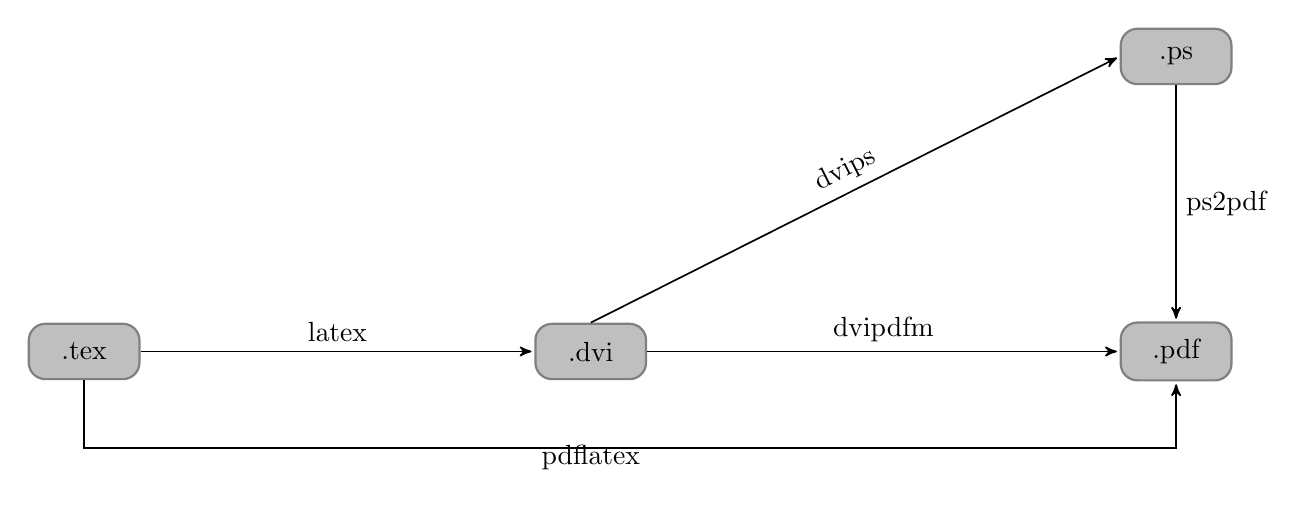
\begin{tikzpicture}
    \node[box] (tex) {.tex};
    \node[box] (dvi) [right=5 of tex] {.dvi};
    \node[box] (pdf) [right=6 of dvi] {.pdf};
    \node[box] (ps) [above=3 of pdf] {.ps};
    \path (tex) edge [arrow] node[auto] {latex} (dvi)
        (dvi) edge [arrow] node[auto] {dvipdfm} (pdf)
        (dvi.north) [arrow,draw] to node[above,sloped] {dvips} (ps.west)
        (ps) edge [arrow] node[right] {ps2pdf} (pdf)
        (tex) edge [arrow,bloop] (pdf);
    \node [below=.7 of dvi] {pdflatex};
\end{tikzpicture}
\caption{格式转换}
\label{fig:convert_format}
\end{figure}

最早的~driver~是~\verb|dvips|,它把~DVI~转换为~PS。\verb|dvipdf|~把~DVI~转为~PDF,它后来被~\verb|dvipdfm|~所取代;\verb|dvipdfm|~主要用于处理单字节字符,1999~年之后停止开发;在~\verb|dvipdfm|~基础上发展来的~\verb|dvipdfmx|~可以处理多字节编码。

pdf\TeX~是一种特殊的driver,它跳过~DVI,直接用~\TeX~源文件生成~PDF。基于~pdf\TeX~的~pdf\LaTeX~则把\LaTeX~源文件转为~PDF。

\verb|dvipdfmx|对图形格式的兼容性较好,而且擅长处理中文。

得到~DVI~后,我们可以在控制台用以下命令把它转为~PDF。
\begin{code}
dvipdfm xxx(.dvi)
\end{code}

我们也可以把它转为~PS,接着用~Ghostscript~的一个命令行程序把它转换为~PDF,注意第二个命令需要~\verb|.ps|~后缀。一般情况下不推荐这种方法,因为它多了个步骤。
\begin{code}
dvips xxx(.dvi)
ps2pdf xxx.ps
\end{code}

pdf\LaTeX~用法如下
\begin{code}
pdflatex xxx(.tex)
\end{code}

\subsection{\LaTeX~语句}
\LaTeX~源文件的每一行称作一条语句(statement),语句可以分三种:命令(command)、数据(data)和注释(comment)。

命令分为两种:普通命令和环境(environment)。普通命令以\verb|\|~起始,大多只有一行;而环境包含一对起始声明和结尾声明,用于多行的场合。命令和环境可以互相嵌套。

\LaTeX~源文件的结构分三大部分,依次为:文档类声明、序言(可选)、正文。
这三部分的基本语法如下:
\begin{code}
\documentclass[options]{class}  %文档类声明
\usepackage[options]{package}   %引入宏包
...
\begin{document}                %正文
...
\end{document}
\end{code}

把下面例子用编辑器保存为~\verb|hello_world.tex|,这就是一个最简单的~\LaTeX~源文件。
%\label{subsec:hello_world}
\begin{code}
%hello_world.tex
\documentclass{article}
\begin{document}
    Hello, World!
\end{document}
\end{code}

\section{\LaTeX~ 中文模版}
\label{sec:template}
下面是一个~\LaTeX~ 中文模版\footnote{这是我找到的模版中最好的一个了,尽管没有涉及到系统命令的更改}, 仅供参考!

\begin{verbatim}
%%%%%%%%%%%%%%%%%%%%%%%%%%%%%%%%%%%
\iffalse                             % 块注释
如果要注释一块文字,用\iffalse ... \fi 界定住要
注释的文字。特别提醒:以下设置的次序不能乱,否则
会引发冲突,影响到编译是否成功。
\fi
\documentclass[a4paper,11pt,         % A4纸
               twoside,              % 双面
%              openany               % 新章节在偶数页开始
               ]{article}

%%%%%%%%%% 版面控制 %%%%%%%%%%
\usepackage{indentfirst}             % 首行缩进
\iffalse
\usepackage[%paperwidth=18.4cm, paperheight= 26cm,
            body={14.6true cm,22true cm},
            twosideshift=0 pt,

 %headheight=1.0true cm
            ]{geometry}
\fi
\usepackage[perpage,symbol]{footmisc}% 脚注控制
\usepackage[sf]{titlesec}            % 控制标题
\usepackage{titletoc}                % 控制目录
\usepackage{fancyhdr}                % 页眉页脚
\usepackage{type1cm}                 % 控制字体大小
\usepackage{indentfirst}             % 首行缩进
\usepackage{makeidx}                 % 建立索引
\usepackage{textcomp}                % 千分号等特殊符号
\usepackage{layouts}                 % 打印当前页面格式
\usepackage{bbding}                  % 一些特殊符号
\usepackage{cite}                    % 支持引用
\usepackage{color,xcolor}            % 支持彩色文本、底色、文本框等
\usepackage{listings}                % 粘贴源代码
\lstloadlanguages{}                  % 所要粘贴代码的编程语言
\lstset{language=,tabsize=4, keepspaces=true,
    xleftmargin=2em,xrightmargin=2em, aboveskip=1em,
    backgroundcolor=\color{lightgray},    % 定义背景颜色
    frame=none,                      % 表示不要边框
    keywordstyle=\color{blue}\bfseries,
    breakindent=22pt,
    numbers=left,stepnumber=1,numberstyle=\tiny,
    basicstyle=\footnotesize,
    showspaces=false,
    flexiblecolumns=true,
    breaklines=true, breakautoindent=true,breakindent=4em,
    escapeinside={/*@}{@*/}
}

%%%%%%%%%% 字体支持 %%%%%%%%%%%%
%\usepackage{ccmap}                  % 使pdfLatex生成的文件支持复制等
\usepackage{CJK,CJKnumb,CJKulem}     % 中文支持
\usepackage{times}     % 包括 Times Roman + Helvetica + Courier
%\usepackage{palatino} % 包括 Palatino + Helvetica + Courier
%\usepackage{newcent} %包括 New Century Schoolbook + Avant Garde + Courier
%\usepackage{bookman}  % 包括 Bookman + Avant Garde + Courier

%%%%%%%%%% 数学符号公式 %%%%%%%%%%
\usepackage{latexsym}
\usepackage{amsmath}                 % AMS LaTeX宏包
\usepackage{amssymb}                 % 用来排版漂亮的数学公式
\usepackage{amsbsy}
\usepackage{amsthm}
\usepackage{amsfonts}
\usepackage{mathrsfs}                % 英文花体字体
\usepackage{bm}                      % 数学公式中的黑斜体
\usepackage{relsize}    % 调整公式字体大小:\mathsmaller, \mathlarger
\usepackage{caption2}                % 浮动图形和表格标题样式

%%%%%%%%%% 图形支持宏包 %%%%%%%%%%
\ifx\pdfoutput\undefined             % 用latex或pdflatex编译
  \usepackage[dvips]{graphicx}       % 将eps格式的图片放在figures目录下
\else                                % 在setup/format.tex中用以下命令注明路径:
  \usepackage[pdftex]{graphicx}      % \graphicspath{{figures/}}
\fi
%\usepackage{subfigure}
\usepackage{epsfig}                  % 支持eps图像
%\usepackage{picinpar}               % 图表和文字混排宏包
%\usepackage[verbose]{wrapfig}       % 图表和文字混排宏包
%\usepackage{eso-pic}                % 向文档的部分页加n副图形, 可实现水印效果
%\usepackage{eepic}                  % 扩展的绘图支持
%\usepackage{curves}                 % 绘制复杂曲线
%\usepackage{texdraw}                % 增强的绘图工具
%\usepackage{treedoc}                % 树形图绘制
%\usepackage{pictex}                 % 可以画任意的图形
%\usepackage{hyperref}

%%%%%%%%%% 一些距离设置 %%%%%%%%%%%
\setlength{\floatsep}{10pt plus 3pt minus 2pt}       % 图形之间或图形与正文之间的距离
\setlength{\abovecaptionskip}{2pt plus 1pt minus 1pt}% 图形中的图与标题之间的距离
\setlength{\belowcaptionskip}{3pt plus 1pt minus 2pt}% 表格中的表与标题之间的距

%%%%%%%%%% 纸张和页面的大小 %%%%%%%%%%
%\paperwidth   20 true cm            % 纸张宽
%\paperheight  30 true cm            % 纸张高
%\textwidth    10 true cm            % 正文宽
%\textheight   20 true cm            % 正文高
%\headheight      14pt               % 页眉高
%\headsep         16pt               % 页眉距离
%\footskip        27pt               % 页脚距离
%\marginparsep    10pt               % 边注区距离
%\marginparwidth  100pt              % 边注区宽
\makeindex                           % 生成索引
\pagestyle{fancy}                    % 页眉页脚风格
\fancyhf{}                           % 清空当前页眉页脚的默认设置

%%%%%%%%%% 导入中文环境 %%%%%%%%%%
\AtBeginDocument{\begin{CJK*}{GBK}{song} % 不计中文的空格
\CJKindent                           % 首行缩进两个汉字
\sloppy\CJKspace                     % 中英文混排的断行
\CJKtilde                            % 重新定义~,用~隔开中英文
\CJKcaption{GB}                      % 章节标题的中文化
}
\AtEndDocument{\end{CJK*}}

%%%%%%%%%% 正文 %%%%%%%%%%
\begin{document}

%%%%%%%%%% 一些新定义 %%%%%%%%%%
\newcommand{\song}{\CJKfamily{song}} % 宋体
\newcommand{\hei}{\CJKfamily{hei}}   % 黑体
\newcommand{\fs}{\CJKfamily{fs}}     % 仿宋
\newcommand{\kai}{\CJKfamily{kai}}   % 楷体

%%%%%%%%%% 定理类环境的定义 %%%%%%%%%%
%% 必须在导入中文环境之后
\newtheorem{example}{例}             % 整体编号
\newtheorem{algorithm}{算法}
\newtheorem{theorem}{定理}[section]  % 按 section 编号
\newtheorem{definition}{定义}
\newtheorem{axiom}{公理}
\newtheorem{property}{性质}
\newtheorem{proposition}{命题}
\newtheorem{lemma}{引理}
\newtheorem{corollary}{推论}
\newtheorem{remark}{注解}
\newtheorem{condition}{条件}
\newtheorem{conclusion}{结论}
\newtheorem{assumption}{假设}

%%%%%%%%%% 一些重定义 %%%%%%%%%%
%% 必须在导入中文环境之后
\renewcommand{\contentsname}{目录}     % 将Contents改为目录
\renewcommand{\abstractname}{摘\ \ 要} % 将Abstract改为摘要
\renewcommand{\refname}{参考文献}      % 将References改为参考文献
\renewcommand{\indexname}{索引}
\renewcommand{\figurename}{图}
\renewcommand{\tablename}{表}
\renewcommand{\appendixname}{附录}
\renewcommand{\proofname}{\hei 证明}
\renewcommand{\algorithm}{\hei 算法}

%%%%%%%%%% 重定义字号命令 %%%%%%%%%%
\newcommand{\yihao}{\fontsize{26pt}{36pt}\selectfont}       % 一号, 1.4倍行距
\newcommand{\erhao}{\fontsize{22pt}{28pt}\selectfont}       % 二号, 1.25倍行距
\newcommand{\xiaoer}{\fontsize{18pt}{18pt}\selectfont}      % 小二, 单倍行距
\newcommand{\sanhao}{\fontsize{16pt}{24pt}\selectfont}      % 三号, 1.5倍行距
\newcommand{\xiaosan}{\fontsize{15pt}{22pt}\selectfont}     % 小三, 1.5倍行距
\newcommand{\sihao}{\fontsize{14pt}{21pt}\selectfont}       % 四号, 1.5倍行距
\newcommand{\bansi}{\fontsize{13pt}{19.5pt}\selectfont}     % 半四, 1.5倍行距
\newcommand{\xiaosi}{\fontsize{12pt}{18pt}\selectfont}      % 小四, 1.5倍行距
\newcommand{\dawu}{\fontsize{11pt}{11pt}\selectfont}        % 大五, 单倍行距
\newcommand{\wuhao}{\fontsize{10.5pt}{10.5pt}\selectfont}   % 五号, 单倍行距

%%%%%%%%%% 页眉和页脚的设置 %%%%%%%%%%
\lhead{一个~\LaTeX+CJK~的简单模板}
\rhead{\TeX~爱好者}
\lfoot{用~\LaTeX~写科技论文}
\rfoot{~\thepage~}

%%%%%%%%%% 论文标题、作者等 %%%%%%%%%%
\title{用~\LaTeX~写科技论文            % 论文标题
      \thanks{这是一个为初学者写的~\LaTeX+CJK~论文模板,未经作者允许可以
      随意下载使用并修改传播,目的是让更多的人迅速上手用~\LaTeX~系统写作。}
       }
\author{于江生\\                     % 作者
        北京大学计算机系}
\date{2008年10月01日}                % 日期
\maketitle                           % 生成标题
\tableofcontents                     % 插入目录
\thispagestyle{empty}                % 首页无页眉页脚

\begin{abstract}
\noindent % 不缩进
\end{verbatim}

这是一个简单的~\LaTeX+CJK~的模板,为~\TeX~的初学者提供便利上手的参照。 %latex notes
\chapter{Linux~笔记}

\begin{center}
\begin{quotation}
假如生活欺骗了你,\\
不要悲伤,不要心急!\\
忧郁的日子里需要镇静。\\
相信吧,快乐的日子将会来临。\\
心儿永远向往着未来;\\
现在却常是忧郁。\\
一切都是瞬息,\\
一切都将会过去;\\
而那过去了的,\\
就会成为亲切的怀恋。\\
\begin{flushright}
---~普希金 《假如生活欺骗了你》
\end{flushright}
\end{quotation}
\end{center}

\section{Swap~的几种宏定义方法}
\label{sec:swap}
\begin{code}
#define swap(x,y)  do{x=x^y;y=x^y;x=x^y;}while(0)

#define swap(x,y)  do{x=x+y;y=x-y;x=x-y;}while(0)

#define swap(x,y)  do{typeof(x) t;t=x;x=y;y=t;}while(0)
\end{code}

以上三种方法均有其缺点,在使用时需酌情处理。对于采用异或方法的,可能会因为变量为有符号数据而出错; 采取算术加减方法的,需要考虑两个参数和或差溢出的可能;而对于~\verb|typeof()|, 可能有些解析器无法解析。

\section{DPRINT~宏实现}
\label{sec:dprint}
\begin{code}
#define  DEBUG

#ifdef DEBUG
#define DPRINT(fmt, args...)  printf(fmt, ##args)
#else
#define DPRINTF(fmt, args...)
#endif
\end{code}

该宏在调试时非常重要,并且使用较为方便,可以对文件中使用的打印输出整体操作。使用时通过改变~\verb|#ifdef|与~\verb|#ifndef|对宏进行开关,其中~\verb|##args|~中的~\#\#~是可变参数的写法。

\section{\#~与~\#\#~使用}
\label{sec:cat}
参数名以~\#~作为前缀则结果将被扩展为由实际参数的带引号的字符串。
\begin{code}
#define SQR(x) printf("the square of #x is %d\n", (x)*(x))
\end{code}
若调用~SQR(8)则输出应该是”the square of 8 is 64“

而对于~\#\#~ 则是把两个语言符号组成单个语言符号
\begin{code}
#define Xcat(x) a##x
\end{code} 
若使用~Xcat(2)~则输出应该是~a2,当然对于一些情况~\#\#~就不具有相应地扩展字符的作用
\begin{code}
 #define cat(x, y)  x##y
\end{code}
当嵌套调用如~\verb|cat(cat(1,2),3)|~时,输出为~\verb|cat(1,2)3|~而不是123。那是因为~\#\#~阻止了外层调用的扩展。如下调整可解决这一状况
\begin{code}
#define xcat(x, y)   cat(x,y)
\end{code}
然后通过~\verb|xcat(xcat(1,2),3)|则可以完成。

\section{/etc~下配置文件介绍}
\begin{verbatim}
SHELL默认文件
/etc/bashrc – bash shell 的系统级默认功能和别名 
/etc/profile – bash shell 的系统级默认值,包括系统级的环境变量 
/etc/passwd – 含有用户的密码和其他信息。Root 用户能够直接修改,但建议用配置工具修改,
例如 passwd 命令。一个损坏的/etc/passwd 很容易令一个 Linux 系统不可用。 
/etc/shadow – 存有 passwd 文件的“shadow”信息。比如:不应被所有人看到的信息。 
/etc/group – 类似/etc/passwd 文件,但是关于用户组的。 
/etc/crontab – 设置“cron” ,意为定期地执行命令(以小时、天、星期、年等为单位)。 
/etc/initab – 系统启动时运行不同的程序和进程。 
/etc/issue – 和登录提示一起出现的信息。常常被 rc.local 脚本覆盖。 
/etc/issue.net – 与上面相同,但是在通过网络登录时使用。 
/etc/motd – “每日消息(Message of the day)”文件,用户登录后显示。 
/etc/rc.d/rc.local – 系统启动时最后执行的脚本。我把定制我的本地机器的命令放在此文件的
末尾。它的功能类似 DOS 的“autoexec.bat”。 
                                    
网络配置 
/etc/hosts – 含有一个主机名和固定 ip 地址列表 
/etc/hosts.allow – 允许使用网络服务的主机名 
/etc/hosts.deny – 禁止使用网络服务的主机名 
/etc/resolv.conf – 设置了本地机器使用的域名服务器列表 
/etc/inetd.conf – 守护进程 inetd 的配置文件,说明了你的机器提供哪些 TCP/IP 服务。 
/etc/exports – 指明了哪些文件系统能想那些主机提供网络文件系统(NFS)。Man exports 包
含如何为远程用户设置此文件的信息。 
 
硬件配置 
/etc/conf.modules – 配置 linux 的核心模块。模块类似 MS Windows 或 DOS 下的设备驱动程序。 
/etc/fstab – 还有分区和文件系统信息。系统用来 mount 目录树上不同的文件系统和分区。 
/etc/mtab – 显示当前以被 mount 的设备和分区,以及它们的状态。 
/etc/lilo.conf – lilo 启动管理程序的配置文件。 
/boot/grub/grub.conf – grub 启动管理程序的配置文件。 
/etc/printcap – 打印机设置 
/etc/termcap – ASCII 数据库,定义了不同控制台、终端和打印机的功能和字符特性。你一般不
会去改变它们。 
/etc/X11/XF86Config – X 配置文件。Xfree 4.xx 版本的配置文件是/etc/X11/XF86Config-4
(如果它不存在,系统会试用 XF86Config)。 
\end{verbatim}

\section{linux~根目录下文件介绍}
\begin{verbatim}
*/proc 是一个虚拟文件系统,可提供内核,硬件和正在运行的进程的详细信息。大多数在/proc下的文件都可以用cat命令进行浏览,但有些使用无效字符来进行内容区分,因此浏览文件的命令不统一。
*/sys  是新版本中添加的文件,其内容和/proc的相似,但对内容作分类处理。
/etc  是系统配置文件存放的目录。
*/bin  是存放可执行文件的目录,如一些常用命令ls,mv,cp等。
*/sbin 也是存放可执行文件的目录,不过这些可执行文件为系统可执行文件,一般用户使用时会有权限限制。
/dev 是存放设备文件的地方,而这些设备文件是由udev管理存放的。这些文件只有在设备接入时才生成,当设备移除后文件自动删除。
*/lib 是存放库文件的目录。 
/boot 存放系统内核和引导文件的目录。
(/proc /sys /dev 下的文件均为动态的,会随着系统环境的改变而改变。/proc /sys mount到多个目录下时其内容均一至,而/dev 会因mount的设备文件不同而不同)
(加*为必需文件目录)
\end{verbatim}

\section{\#error~与~\#warn}
一般编译较小的程序时不加入这两个调试语句,但当编译较大的程序时使用这两个语句就显得很方便了。一般将其加入到多分支的语句中。

区别:
在编译时如遇到~\#error~就会退出编译,如果遇到~\#warn~仅会发出警示语句,但编译仍在进行。

\section{the process of compile}

\begin{figure}[htbp]
\centering
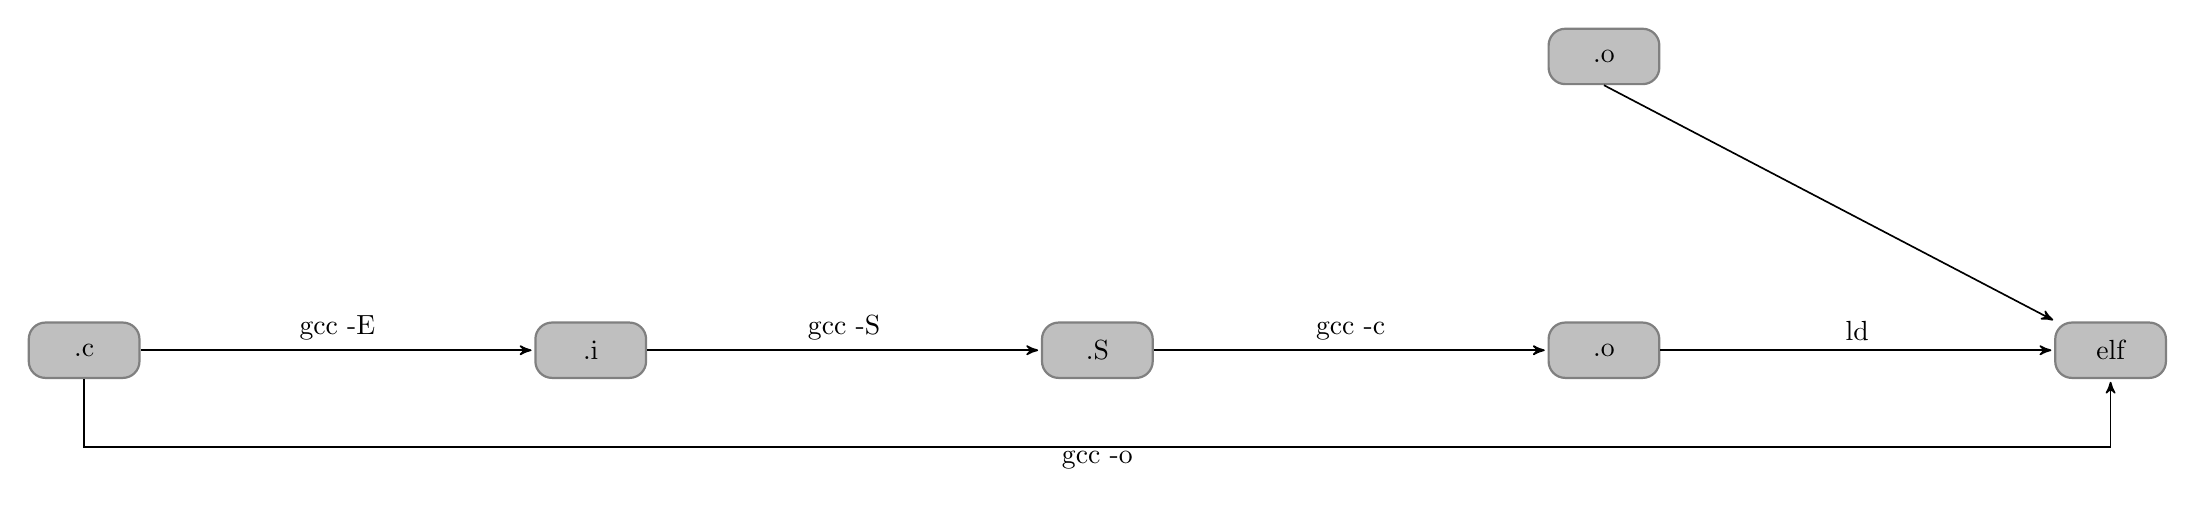
\begin{tikzpicture}
    \node[box] (c) {.c};
    \node[box] (i) [right=5 of c] {.i};
    \node[box] (s) [right=5 of i] {.S};
    \node[box] (o-c) [right=5 of s] {.o};
    \node[box] (o-a) [above=3 of o-c] {.o};
    \node[box] (elf) [right=5 of o-c] {elf};
    \path (c) edge [arrow] node[auto] {gcc -E} (i)
        (i) edge [arrow] node[auto] {gcc -S} (s)
        (s) edge [arrow] node[auto] {gcc -c} (o-c)
        (o-c) edge [arrow] node[auto] {ld} (elf)
        (o-a.south) [arrow,draw] to node[auto] {} (elf)
        (c) edge [arrow,bloop] (elf);
    \node [below=.8 of s] {gcc -o};
\end{tikzpicture}
\caption{格式转换}
\label{fig:convert_format}
\end{figure}

\section{\textless \textgreater and ""}
when we \#include \verb|<|headfile.h\verb|>|, it just search headfile at standard route.but if it is \#include "headfile.h",it will search headfile at currently route,then the standard route

\section{操作系统的主要作用}
操作系统是一个庞大的管理控制程序,大致包括5个方面的管理功能:
\begin{itemize}
	\item Thread management 
	\item Device management
	\item Memory management
	\item User interface (I/O)
	\item File system
\end{itemize}

Memory management :1.内存的分配与释放 2.内存的共享与保护着 3.虚拟地址与物理地的映射 4.虚拟内存

其中最核心的功能是进程管理,但基础是内存管理。

系统工作模式有三种:实模式、保护模式、虚拟8086模式,

其中保护模式又分为:分段保护模式、分段分页保护模式,不同模式下的物理内存管理方式不同。

堆栈段存放的就是子程序的返回地址、子程序的参数以及程序的局部变量。

数据段则存放程序的全局变量,常数以及动态数据分配的数据空间

\section{对于MMU的简单理解}
X86~平台的虚拟空间是0x00000000\~{}0xffffffff,大致上前~3G(0x0000000\~{}0xbfffffff)~是用户空间,后~1G(0xc0000000\~{}0xffffffff)~是内核空间。0x0804 8000\~{}0x080f 4000是从~/bin/bash~加载到内存的,访问权限为~r-x,表示~Text Segment,包含.text~段、.rodata~段、.plt~段等。0x080f 4000\~{}0x080f 9000也是从~/bin/bash~加载到内存的,访问权限为~rw-,表示~Data Segment~,包含.data~段、.bss~段等。

0x0928 3000\~{}0x0949 7000~不是从磁盘中加载到内存中的,这段空间称为堆。

虚拟内存管理的作用:
\begin{itemize}
	\item  虚拟内存管理可以控制物理内存的访问权限。物理内存本身是不限制访问权限的,任何地址都是可读写的。而操作系统要求不同的页面要具有不同的访问权限。这就利用CPU模式和MMU的内存保护机制实现。
	\item  虚拟内存管理最主要的作用是让每个进程有独立的地址空间。所谓独立的地址空间是指,不同的进程中的同一个虚拟地址被MMU映射到不同的物理地址,并且在某一进程中访问任何地址都不可能访问另外一个进程的数据,这样使得因任意一进程执行过程中恶意代码导致的非法内存访问不会影响其他进程的运行,从而保证了整个系统的稳定性。
	\item  从虚拟地址到物理地址的映射会给分配内存带来极大的方便,物理地址不连续的几块内存可以映射成虚拟地址连续的一块内存。这样就可以分配多个不连续的物理页面而映射到连续的虚拟地址范围。
	\item  一个系统如果同时运行着很多进程,为各进程分配的内存之和可能会大于实际可用的物理内存,虚拟内存管理使得这种情况下各个进程仍能够正常运行。因为各进程分配的的只不过是虚拟内存页面,这些页面的数据可以映射到物理页面,也可以临时保存到磁盘上而不占用物理页面。
\begin{code}
系统可分配的内存总量 = 物理内存大小 + 交换设备大小(swap)}
\end{code}
\end{itemize}

\section{ARM}
\subsection{体系结构中的几个基本概念}
\textbf{三个级别}
\begin{itemize}
	\item Board(开发板级)
	\item SOC(片上系统级)
	\item CPU级
\end{itemize}

\textbf{不同的ARM处理器之间的区别}
\begin{itemize}
	\item CPU core 或者协处理器不同(按需求,如同一个版本即可以支持浮点运算,也可以不支持)
	\item 流水线级数不同(ARM version越高流水线越多)
	\item cache大小不同(version 越高cache越多)
\end{itemize}

\subsection{ARM family}
\begin{table}[htbp]
\label{tab:arm family}
\centering 
\begin{tabular}{|l|l|}
\hline
Architecture & Family \\\hline
ARMv1 & ARM1 \\\hline
ARMv2 & ARM2, ARM3 \\\hline
ARMv3 & ARM6, ARM7 \\\hline
ARMv4 & StrongARM, ARM7TDMI, ARM9TDMI \\\hline
ARMv5 & ARM7EJ, ARM9E, ARM10E, XScale \\\hline
ARMv6 & ARM11 \\\hline
ARMv7 & cortex \\\hline
\end{tabular}
\caption{ARM family}
\end{table}

\subsection{ARM体系结构}
\textbf{Architecture}
\begin{itemize}
	\item mode
	\item register
	\item instrction
	\item mmu
	\item pipe line
	\item irq
	\item cache
\end{itemize}

\textbf{Exception Modes}
\begin{itemize}
	\item FIQ
	\item IRQ
	\item Supervisor
	\item Abort
	\item Undefined
\end{itemize}

\textbf{Processor Modes}\\
The ARM architecture supports seven processor modes\\
\begin{tabular}{|l|c|l|}
\hline
Processor  & mode & Description   \\\hline
User & usr & Normal program execution mode \\\hline
FIQ& fiq & supports a high-speed data transfe or channel process \\\hline
IRQ & irq & Used for general-purpose interrupt handling \\\hline
Supervisor& svc & A protected mode for the opeerating system \\\hline
Abort& abt & Implements virtual memory and/or memory protection \\\hline
Undefined& und & Supports software emulation of hardware coprocessors \\\hline
System& sys & Runs privileged operating system tasks(ARMv4 and above) \\\hline
\end{tabular}

\subsection{Data}
\begin{code}
	Byte  8bits
	Halfword  16bits
	Word 32bits
\end{code}
ARMv6 introduced a variety of Single Instruction Multiple Data (SIMD) instructions
operating on two halfwords or four bytes in parallel.\\
ARM instructions are exactly one word and are aligned on a four-byte boundary. Thumb instructions
are exactly one halfword and are aligned on a two-byte boundary. Jazelle opcodes are a variable
number of bytes in length and can appear at any byte alignment.

\subsection{Register}
\noindent The ARM processor has a total of 37 registers:\\
Thirty-one general-purpose registers, including a program counter. These registers are 32 bits wideand are described in General-purpose registers \\
Six status registers. These registers are also 32 bits wide, but only some of the 32 bits are allocated or need to be implemented. The subset depends on the architecture variant supported. These are described in Program status registers\\
\begin{code}
R13通常是sp(栈指针),R14是PC指针,R15是CPSR
\end{code}

\textbf{Program status registers}\\ 
The Current Program Status Register (CPSR) is accessible in all processor modes. It contains condition code flags, interrupt disable bits, the current processor mode, and other status and control information. Each exception mode also has a Saved Program Status Register (SPSR), that is used to preserve the value of the CPSR when the associated exception occurs.\\
The format of the CPSR and the SPSRs:\\
\begin{tabular}{|c|c|c|c|c|c|c|c|c|c|c|c|c|c|c|c|}
\hline
N&Z&C&V&Q&Res&J&Res&GE[3:0]&Res&E&A&I&F&T&M[4:0]\\
\hline
\end{tabular}

\textbf{The condition code flags}\\
\begin{description}
\item[N] is set to bit 31 of the result of the instruction. If this result is regarded as a two's complement signed integer, then N = 1 if the result is negative and N = 0 if it is positive or zero.
\item[Z] is set to 1 if the result of the instruction is zero (this often indicates an equal result from a comparison), and to 0 otherwise.
\item[C] 
\begin{itemize}
\item For an addition, including the comparison instruction CMN, C is set to 1 if the addition
produced a carry (that is, an unsigned overflow), and to 0 otherwise.
\item For a subtraction, including the comparison instruction CMP, C is set to 0 if the
subtraction produced a borrow (that is, an unsigned underflow), and to 1 otherwise.
\item For non-addition/subtractions that incorporate a shift operation, C is set to the last bit
shifted out of the value by the shifter.
\item For other non-addition/subtractions, C is normally left unchanged (but see the
individual instruction descriptions for any special cases).
\end{itemize} 
\item{V} 
\begin{itemize}
\item For an addition or subtraction, V is set to 1 if signed overflow occurred, regarding the
operands and result as two's complement signed integers.
\item For non-addition/subtractions, V is normally left unchanged (but see the individual
instruction descriptions for any special cases).
\end{itemize}
\end{description}

\textbf{The interrupt disable bits}\\
\begin{description}
\item[A] Disables imprecise data aborts when it is set. This is available only in ARMv6 and above.
In earlier versions, bit[8] of CPSR and SPSRs must be treated as a reserved bit, as described
in Types of PSR bits.
\item[I] Disables IRQ interrupts when it is set
\item[F] Disables FIQ interrupts when it is set.
\end{description}
\textbf{Tips}:we can see the man page,page two is system call and page three is the libc

\subsection{asm code}
\textbf{add from a number to another}
\begin{code}
	.text
	.global sum

sum:
	stmfd sp!, {r4-r7, lr}
	mov r2, #0

loop:
	add r2, r0, r2
	add r0, r0, #1
	cmp r0, r1
	bne loop

	add r2, r2, r0
	mov r0, r2

	ldmfd sp!, {r4-r7, pc}
\end{code}

\section{Vim~的使用}
\indent 在不同工作模式下使用~VIM~的一些基本技巧——即插入模式(insert mode), 命令模式(command mode), 存取文件等。在这篇文章里面,代表~Ctrl + X~——就是按住~Ctrl~键然后再按~X。而且你可以在很多情况下使用 :help command 来获得大部分命令的帮助,这个是 VIM 的内部帮助文件命令。

\subsection{高效率移动}
在插入模式之外基本上来说,你应该尽可能少的呆在插入模式里面,因为在插入模式里面 VIM 就像一个“哑巴”编辑器一样。很多新手都会一直呆在插入模式里面,因为这样易于使用。但 VIM 的强大之处在于他的命令行模式!你会发现,在你越来越了解 VIM 之后,你就会花越来越少的时间使用插入模式了。

\textbf{使用 h、j、k、l}\\
使用 VIM 高效率编辑的第一步,就是放弃使用箭头键。使用 VIM,你就不用频繁的在箭头键和字母键之间移来移去了,这会节省你很多时间。当你在命令模式时,你可以用 h、j、k、l 来分别实现左、下、上、右箭头的功能。一开始可能需要适应一下,但一旦习惯这种方式,你就会发现这样操作的高效之处了。
在你编辑你的电子邮件或者其他有段落的文本时,你可能会发现使用方向键和你预期的效果不一样,有时候可能会一次跳过了很多行。这是因为你的段落在 VIM 看来是一个大的长长的行。这时你可以在按 h、j、k 或者 l 之前键入一个 g,这样 VIM 就会按屏幕上面的行如你所愿的移动了。

\textbf{在当前行里面有效的移动光标}\\
很多编辑器只提供了简单的命令来控制光标的移动(比如左、上、右、下、到行首/尾等)。VIM 则提供了很多强大的命令来满足你控制光标的欲望。当光标从一点移动到另外一点,在这两点之间的文本(包括这两个点)称作被“跨过”,这里的命令也被称作是 motion。(简单说明一下,后面会用到这个重要的概念)
这里是常用到的一些命令(motion):
\begin{description}
	\item[fx]:移动光标到当前行的下一个 x 处。很明显,x 可以是任意一个字母,而且你可以使用 ; 来重复你的上一个 f 命令。
	\item[tx]:和上面的命令类似,但是是移动到 x 的左边一个位置。(这真的很有用)
	\item[Fx]:和 fx 类似,不过是往回找。
	\item[w]:光标往前移动一个词。
	\item[b]:光标往后移动一个词。 
	\item[0]:移动光标到当前行首。 
	\item[\^{}]:移动光标到当前行的第一个字母位置。 
	\item[\$]:移动光标到行尾。 
	\item[\symbol{'50}]:移动光标到下一个句子。 
	\item[\symbol{'51}]:移动光标到上一个句子。
\end{description}
 
\textbf{在整个文件里面有效移动光标}\\
VIM~有很多命令,可以用来到达文件里面你想到达的地方。下面是一些在文件里面移动的命令:
\begin{description}
	\item[ctrl+f]:向下移动一屏。
	\item[ctrl+b]:向上移动一屏。
	\item[G]:到文件尾 
	\item[numG]:移动光标到指定的行(num)。(比如 10G 就是到第 10 行)
	\item[gg]:到文件首
	\item[H]:移动光标到屏幕上面
	\item[M]:移动光标到屏幕中间 
	\item[L]:移动光标到屏幕下面
	\item[*]:读取光标处的字符串,并且移动光标到它再次出现的地方。
	\item[\#{}]:和上面的类似,但是是往反方向寻找。
	\item[/text]:从当前光标处开始搜索字符串 text,并且到达 text 出现的地方。必须使用回车来开始这个搜索命令。如果想重复上次的搜索的话,按 n。
	\item[?text]:和上面类似,但是是反方向。
	\item[ma]:在当前光标的位置标记一个书签,名字为 a。书签名只能是小写字母。你看不见书签的存在,但它确实已经在那里了。
	\item[\`{}a]:到书签 a 处。注意这个不是单引号,它一般位于大部分键盘的 1 的左边。
	\item[\`{}.]:到你上次编辑文件的地方。这个命令很有用,而且你不用自己去标记它。
\end{description}

\subsection{高效的输入}
\textbf{使用关键词自动完成}\\
VIM 有一个非常漂亮的关键词自动完成系统。这表示,你可以输入一个长词的一部分,然后按一下某个键,然后 VIM 就替你完成了这个长词的输入了。举个例子:你有一个变量名为 iAmALongAndAwkwardVarName 在你写的代码的某个地方。也许你不想每回都自己一个一个字母的去输入它。\\
使用关键词自动完成功能,你只需要输入开始几个字母(比如 iAmAL),然后按 (按住 Ctrl,再按 N)或者 。如果 VIM 没有给出你想要的词,继续按,直到你满意为止,VIM 会一直循环它找到的匹配的字符串。

\textbf{聪明的进入插入模式}\\
很多新手进入插入模式都只是用 i。这样当然可以进入插入模式,但通常不是那么合适,因为 VIM 提供了很多进入插入模式的命令。下面是最常用的一些:
\begin{description}
 	\item[i]:在当前字符的左边插入 
 	\item[I]:在当前行首插入
 	\item[a]:在当前字符的右边插入 
 	\item[A]:在当前行尾插入 
 	\item[o]:在当前行下面插入一个新行
 	\item[O]:在当前行上面插入一个新行
 	\item[c\{motion\}]:删除 motion 命令跨过的字符,并且进入插入模式。比如:c\$,这将会删除从光标位置到行尾的字符并且进入插入模式。ct!,这会删除从光标位置到下一个叹号(但不包括),然后进入插入模式。被删除的字符被存在了剪贴板里面,并且可以再粘贴出来。
 	\item[d\{motion\}]:和上面差不多,但是不进入插入模式。
\end{description}
 
\textbf{有效的移动大段的文本} \\
使用可视选择(visual selections)和合适的选择模式
不像最初的 VI,VIM 允许你高亮(选择)一些文本,并且进行操作。这里有三种可视选择模式:
\begin{description}
	\item[v]:按字符选择。经常使用的模式,所以亲自尝试一下它。
	\item[V]:按行选择。这在你想拷贝或者移动很多行的文本的时候特别有用。
	\item[$<$C-V$>$]:按块选择。非常强大,只在很少的编辑器中才有这样的功能。你可以选择一个矩形块,并且在这个矩形里面的文本会被高亮。
\end{description}
在选择模式的时候使用上面所述的方向键和命令(motion)。比如,vwww,会高亮光标前面的三个词。Vjj将会高亮当前行以及下面两行。

\textbf{在可视选择模式下剪切和拷贝}\\
一旦你高亮了选区,你或许想进行一些操作:
\begin{description}
	\item[d]:剪贴选择的内容到剪贴板。
	\item[y]:拷贝选择的内容到剪贴板。
	\item[c]:剪贴选择的内容到剪贴板并且进入插入模式。
\end{description}

\textbf{在非可视选择模式下剪切和拷贝}\\ 
如果你很清楚的知道你想拷贝或者剪切什么,那你根本就不需要进入可视选择模式。这样也会节省时间:
\begin{description}
	\item[d\{motion\}]:剪切motion命令跨过的字符到剪贴板。比如,dw会剪切一个词而dfS会将从当前光标到下一个S之间的字符剪切至剪贴板。
	\item[y\{motion\}]:和上面类似,不过是拷贝。
	\item[c\{motion\}]:和d\{motion\}类似,不过最后进入插入模式。
	\item[dd]:剪切当前行
	\item[yy]:拷贝当前行
	\item[cc]:剪切当前行并且进入插入模式
	\item[D]:剪切从光标位置到行尾到剪贴板
	\item[Y]:拷贝当前行
	\item[C]:和D类似,最后进入插入模式。
	\item[x]:剪切当前字符到剪贴板
	\item[s]:和x类似,不过最后进入插入模式
\end{description}

\textbf{粘贴}\\
粘贴很简单,按p。

\textbf{使用多重剪贴板}\\
很多编辑器都只提供了一个剪贴板。VIM有很多。剪贴板在VIM里面被称为寄存器(Registers)。你可以列出当前定义的所有寄存器名和它们的内容,命令为":reg"。最好使用小写字母来作为寄存器的名称,因为大写的有些被VIM占用了。

使用寄存器的命令为双引号“。

比如:我们要拷贝当前行到寄存器k。你应该按 "kyy。(你也可以使用 V"ky。为什么这样也可以呢?)现在当前行应该已经存在了寄存器k里面直到你又拷贝了一些东西进入寄存器k。现在你可以使用命令 "kp 来粘贴寄存器k里面的内容到你想要的位置。

\subsection{避免重复}
\textbf{令人惊奇的 . 命令}\\
在VI里面,输入 . (小数点符号),将会重复你给入的上一个命令。比如,你上个命令为 'dw'(删除一个词),VI将会接着再删除一个词。

\textbf{使用数字}\\
使用数字也是VIM强大的而且很节省时间的重要特性之一。在很多VIM的命令之前都可以使用一个数字,这个数字将会告诉VIM这个命令需要执行几次。比如:
\begin{verbatim}
3j 将会把光标向下移动三行。

10dd 将会删除十行。

y3" 将会拷贝从当前光标到第三个出现的引号之间的内容到剪贴板。
\end{verbatim}
数字是扩展motion命令作用域非常有效的方法。

\textbf{记录宏} 
有时候,你会发现你自己在文章的每段或者每行都重复相同的一系列动作。VIM允许你记录一个宏来完成你的特殊需要。
\begin{verbatim}
qregister:记录宏到寄存器register,这里register是任意的你的寄存器的名字。比如qa,将会记录并且把宏存在寄存器a里面。

q:结束宏的记录。

@register:使用存在寄存器register的宏。比如@a,将会使用存在寄存器a里面的宏。
\end{verbatim}
必须要记住的是,宏只记录了你的系列按键并且重复执行它们。它们不是魔法。因为在VIM里面完成目的的方法有很多,所以有时候你要小心选择命令来记录你的宏。因为它们会在所有你要执行它的地方执行。

\subsection{用VIM写代码}
VIM是一个绝好的编辑器来写代码,因为它有一些特性是专门为程序员而设。这里是一些常用的:
\begin{description}
	\item[\symbol{'135}p]:和p的功能差不多,但是它会自动调整被粘贴的文本的缩进去适应当前代码的位置。试一下!
	\item[\%]:匹配花括号,方括号,括号等。在一个括号的上面,然后按\%,鼠标就会出现在匹配的另外一半括号处。
	\item[\textgreater\textgreater]:缩进所有选择的代码
	\item[\textless\textless]:和上面类似,但是反缩进
	\item[gd]:到达光标所在处函数或者变量的定义处
	\item[K]:在Man里面查找光标当前所在处的词。
\end{description}

\subsection{Vim~中的一个替换实例}
\begin{code}
write(AAAA, BBBB);
	|
	|
	V
write(VA(AAAA), BBBB);

:%s/\(write(\)\(.*\)\(,.*\)/\1VA\(\2\)\3/g
\end{code}

\section{汇编文件命名中s与S的区别}
以.S命名的汇编文件可以用一些C语言中的属性,比如添加一些头文件和一些宏定义等,而以.s命名的就没有这些属性。

\section{Makefile}
\begin{code}
将所有.c 文件编译,编译指定生成 elf 文件和本文件名一样(去掉.c),并且有 make clean 的功能

SRC = $(wildcard *.c)

OBJ =  $(SRC:%.C = %)

$(OBJ):
    for pkg in $(OBJ);
    do \
        gcc -o $$pkg $$pkg.c;\
    done
clean: $(OBJ)

    rm -vf  $(OBJ) 
\end{code}

\section{如何生成pubkey}
\begin{verbatim}
1. 先执行如下命令
sh-keygen (一路回车)

2. 复制,同时更名
$ fs=”~/.ssh/id_rsa.pub”
$ fd=`awk ‘{print $3}’ $fs`
$ fd=$fd.pub
$ cp –v $fs $fd
\end{verbatim}

\section{shell~中一些命令的用法}
\begin{verbatim}
1)判断表达式 

if test  (表达式为真)

if test !表达式为假

test 表达式1 –a 表达式2                  两个表达式都为真

test 表达式1 –o 表达式2                 两个表达式有一个为真

 
2)判断字符串

test –n 字符串                                   字符串的长度非零

test –z 字符串                                    字符串的长度为零

test 字符串1=字符串2                    字符串相等

test 字符串1!=字符串2               字符串不等

 
3)判断整数

test 整数1 –eq 整数2                        整数相等

test 整数1 –ge 整数2                        整数1大于等于整数2

test 整数1 –gt 整数2                         整数1大于整数2

test 整数1 –le 整数2                         整数1小于等于整数2

test 整数1 –lt 整数2                          整数1小于整数2

test 整数1 –ne 整数2                        整数1不等于整数2

 
4)判断文件

test  File1 –ef  File2                            两个文件具有同样的设备号和i结点号

test  File1 –nt  File2                            文件1比文件2 新

test  File1 –ot  File2                            文件1比文件2 旧

test –b File                 文件存在并且是块设备文件

test –c File                 文件存在并且是字符设备文件

test –d File                 文件存在并且是目录

test –e File                 文件存在

test –f File                 文件存在并且是正规文件

test –g File                 文件存在并且是设置了组ID

test –G File                 文件存在并且属于有效组ID

test –h File                 文件存在并且是一个符号链接(同-L)

test –k File                 文件存在并且设置了sticky位

test –b File                 文件存在并且是块设备文件

test –L File                 文件存在并且是一个符号链接(同-h)

test –o File                 文件存在并且属于有效用户ID

test –p File                 文件存在并且是一个命名管道

test –r File                 文件存在并且可读

test –s File                 文件存在并且是一个套接字

test –t FD                   文件描述符是在一个终端打开的

test –u File                 文件存在并且设置了它的set-user-id位

test –w File                 文件存在并且可写

test –x File                 文件存在并且可执行
\end{verbatim}

\section{软件开发常用词汇}
\begin{verbatim}
A
abstract   抽象的
abstract base class (ABC)抽象基类
abstract class 抽象类
abstraction 抽象、抽象物、抽象性
access 存取、访问
access function 访问函数
access level访问级别
account 账户
action   动作
activate 激活
active   活动的
actual parameter 实参
adapter 适配器
add-in 插件
address 地址
address space     地址空间
ADO(ActiveX Data Object)ActiveX数据对象
advanced    高级的
aggregation 聚合、聚集
algorithm 算法
alias 别名
align 排列、对齐
allocate 分配、配置
allocator分配器、配置器
angle bracket 尖括号
annotation   注解、评注
API (Application Programming Interface) 应用(程序)编程接口
appearance 外观
append     附加
application 应用、应用程序
application framework 应用程序框架
Approximate String Matching 模糊匹配
architecture 架构、体系结构
archive file 归档文件、存档文件
argument参数。
array   数组
arrow operator 箭头操作符
assert(ion) 断言
assign      赋值
assignment 赋值、分配
assignment operator 赋值操作符
associated 相关的、相关联的
asynchronous 异步的
attribute   特性、属性
authentication service 验证服务
authorization 授权
B
background   背景、后台(进程)
backup   备份
backup device备份设备
backup file 备份文件
backward compatible    向后兼容、向下兼容
base class 基类
base type 基类型
batch   批处理
BCL (base class library)基类库
Bin Packing 装箱问题
binary 二进制
binding 绑定
bit 位
bitmap 位图
block 块、区块、语句块
boolean 布林值(真假值,true或false)
border 边框
bounds checking 边界检查
boxing 装箱、装箱转换
brace (curly brace) 大括号、花括号
bracket (square brakcet) 中括号、方括号
breakpoint 断点
browser applications 浏览器应用(程序)
browser-accessible application 可经由浏览器访问的应用程序
bug 缺陷错误
build 编连(专指编译和连接)
built-in 内建、内置
bus 总线
business 业务、商务(看场合)
business Logic 业务逻辑
business rules 业务规则
buttons 按钮
by/through 通过
byte 位元组(由8 bits组成)
C
cache 高速缓存
calendar 日历
Calendrical Calculations 日期
call 调用
call operator 调用操作符
callback 回调
candidate key 候选键 (for database)
cascading delete 级联删除 (for database)
cascading update 级联更新 (for database)
casting   转型、造型转换
catalog   目录
chain     链(function calls)
character 字符
character format 字符格式
character set     字符集
check box 复选框
check button 复选按钮
CHECK constraints CHECK约束 (for database)
checkpoint 检查点 (for database)
child class 子类
CIL (common intermediate language)通用中间语言、通用中介语言
class    类
class declaration 类声明
class definition   类定义
class derivation list 类继承列表
class factory    类厂
class hierarchy 类层次结构
class library    类库
class loader     类装载器
class template   类模板
class template partial specializations 类模板部分特化
class template specializations         类模板特化
classification 分类
clause 子句
cleanup   清理、清除
CLI (Common Language Infrastructure)   通用语言基础设施
client 客户、客户端
client application 客户端应用程序
client area 客户区
client cursor 客户端游标 (for database)
client-server 客户机/服务器、客户端/服务器
clipboard 剪贴板
clone 克隆
CLS (common language specification) 通用语言规范
code access security 代码访问安全
code page 代码页
COFF (Common Object File Format)    通用对象文件格式
collection 集合
COM (Component Object Model) 组件对象模型
combo box 组合框
command line 命令行
comment 注释
commit   提交 (for database)
communication 通讯
compatible 兼容
compile time 编译期、编译时
compiler 编译器
component组件
composite index 复合索引、组合索引 (for database)
composite key 复合键、组合键 (for database)
composition   复合、组合
concept 概念
concrete具体的
concrete class 具体类
concurrency 并发、并发机制
configuration 配置、组态
Connected Components 连通分支
connection    连接 (for database)
connection pooling 连接池
console    控制台
constant   常量
Constrained and Unconstrained Optimization 最值问题
constraint 约束 (for database)
construct 构件、成分、概念、构造(for language)
constructor (ctor) 构造函数、构造器
container 容器
containment包容
context 环境、上下文
control 控件
cookie
copy    拷贝
CORBA   通用对象请求中介架构(Common Object Request Broker Architecture)
cover   覆盖、涵盖
create/creation    创建、生成
crosstab query     交叉表查询 (for database)
Cryptography 密码
CTS (common type system)通用类型系统
cube   多维数据集 (for database)
cursor 光标
cursor 游标 (for database)
custom 定制、自定义
D
data   数据
data connection   数据连接 (for database)
data dictionary 数据字典 (for database)
data file 数据文件 (for database)
data integrity 数据完整性 (for database)
data manipulation language (DML)数据操作语言(DML) (for database)
data member   数据成员、成员变量
data source   数据源 (for database)
Data source name (DSN) 数据源名称(DSN) (for database)
data structure数据结构
Data Structures 基本数据结构
data table    数据表 (for database)
data-bound       数据绑定 (for database)
database 数据库 (for database)
database catalog 数据库目录 (for database)
database diagram 数据关系图 (for database)
database file     数据库文件 (for database)
database object   数据库对象 (for database)
database owner    数据库所有者 (for database)
database project 数据库工程 (for database)
database role     数据库角色 (for database)
database schema 数据库模式、数据库架构 (for database)
database script 数据库脚本 (for database)
datagram    数据报文
dataset   数据集 (for database)
dataset       数据集 (for database)
DBMS (database management system)数据库管理系统 (for database)
DCOM (distributed COM)分布式COM
dead lock 死锁 (for database)
deallocate 归还
debug      调试
debugger   调试器
decay      退化
declaration 声明
default     缺省、默认值
DEFAULT constraint默认约束 (for database)
default database 默认数据库 (for database)
default instance 默认实例 (for database)
default result set 默认结果集 (for database)
defer       推迟
definition 定义
delegate    委托
delegation 委托
deploy       部署
derived class 派生类
design pattern 设计模式
destroy   销毁
destructor(dtor)析构函数、析构器
device   设备
DHTML (dynamic HyperText Markup Language)动态超文本标记语言
dialog   对话框
Dictionaries 字典
digest   摘要
digital 数字的
directive (编译)指示符
directory 目录
disassembler 反汇编器
DISCO (Discovery of Web Services)Web Services的查找
dispatch 调度、分派、派发
distributed computing 分布式计算
distributed query     分布式查询 (for database)
DNA (Distributed interNet Application) 分布式网间应用程序
document 文档
DOM (Document Object Model)文档对象模型
dot operator (圆)点操作符
double-byte character set (DBCS)双字节字符集(DBCS)
driver 驱动(程序)
DTD (document type definition) 文档类型定义
dump       转储
dump file 转储文件
E
e-business   电子商务
efficiency 效率
efficient 高效
encapsulation   封装
end user 最终用户
end-to-end authentication 端对端身份验证
engine   引擎
entity 实体
enum (enumeration) 枚举
enumerators 枚举成员、枚举器
equal       相等
equality    相等性
equality operator 等号操作符
error log   错误日志 (for database)
escape character 转义符、转义字符
escape code 转义码
evaluate 评估
event    事件
event driven 事件驱动的
event handler 事件处理器
evidence 证据
exception 异常
exception declaration 异常声明
exception handling 异常处理、异常处理机制
exception specification 异常规范
exception-safe 异常安全的
exit     退出
explicit 显式
explicit specialization 显式特化
explicit transaction 显式事务 (for database)
export      导出
expression 表达式
F
fat client 胖客户端
feature     特性、特征
fetch 提取
field 字段 (for database)
field 字段(java)
field length 字段长度 (for database)
file   文件
filter 筛选 (for database)
finalization 终结
finalizer 终结器
firewall 防火墙
flag     标记
flash memory 闪存
flush 刷新
font 字体
foreign key (FK) 外键(FK) (for database)
form   窗体
formal parameter 形参
forward declaration 前置声明
forward-only 只向前的
forward-only cursor 只向前游标 (for database)
framework 框架
full specialization 完全特化
function 函数
function call operator (即operator ()) 函数调用操作符
function object 函数对象
function template函数模板
functionality    功能
functor 仿函数
G
GC (Garbage collection)     垃圾回收(机制)、垃圾收集(机制)
generate 生成
generic 泛化的、一般化的、通用的
generic algorithm通用算法
genericity 泛型
getter (相对于 setter)取值函数
global        全局的
global object 全局对象
grant       授权 (for database)
group       组、群
group box   分组框
GUI   图形界面
GUID (Globally Unique Identifier) 全球唯一标识符
H
handle     句柄
handler    处理器
hard disk 硬盘
hard-coded 硬编码的
hard-copy 截屏图
hardware   硬件
hash table 散列表、哈希表
header file头文件
heap       堆
help file 帮助文件
hierarchical data 阶层式数据、层次式数据
hierarchy 层次结构、继承体系
high level 高阶、高层
hook   钩子
Host (application)宿主(应用程序)
hot key   热键
HTML (HyperText Markup Language) 超文本标记语言
HTTP (HyperText Transfer Protocol) 超文本传输协议
HTTP pipeline HTTP管道
hyperlink 超链接
I
icon   图标
IDE (Integrated Development Environment)集成开发环境
identifier 标识符
IDL (Interface Definition Language)    接口定义语言
idle time 空闲时间
if and only if当且仅当
IL (Intermediate Language) 中间语言、中介语言
image 图象
IME   输入法
immediate base      直接基类
immediate derived   直接派生类
immediate updating 即时更新 (for database)
implement      实现
implementation 实现、实现品
implicit       隐式
implicit transaction隐式事务 (for database)
import         导入
incremental update 增量更新 (for database)
Independent Set 独立集
index          索引 (for database)
infinite loop       无限循环
infinite recursive 无限递归
information      信息
inheritance      继承、继承机制
initialization   初始化
initialization list 初始化列表、初始值列表
initialize      初始化
inline           内联
inline expansion 内联展开
inner join      内联接 (for database)
instance        实例
instantiated    具现化、实体化(常应用于template)
instantiation   具现体、具现化实体(常应用于template)
integrate       集成、整合
integrity       完整性、一致性
integrity constraint完整性约束 (for database)
interacts 交互
interface 接口
interoperability 互操作性、互操作能力
interpreter   解释器
introspection 自省
invariants    不变性
invoke        调用
isolation level 隔离级别 (for database)
item      项、条款、项目
iterate   迭代
iteration 迭代(回圈每次轮回称为一个iteration)
iterative 反复的、迭代的
iterator 迭代器
J
JIT compilation JIT编译即时编译
Job Scheduling 工程安排
K
key          键 (for database)
key column   键列 (for database)
L
left outer join 左向外联接 (for database)
level      阶、层例
library    库
lifetime   生命期、寿命
Linear Programming 线性规划
link       连接、链接
linkage    连接、链接
linker     连接器、链接器
list   列表、表、链表
list box 列表框
literal constant 字面常数
livelock 活锁 (for database)
load   装载、加载
load balancing 负载平衡
loader 装载器、载入器
local 局部的
local object    局部对象
lock 锁
log   日志
login 登录
login security mode登录安全模式 (for database)
lookup table   查找表 (for database)
loop           循环
loose coupling 松散耦合
lvalue         左值
M
machine code   机器码、机器代码
macro        宏
maintain     维护
managed code 受控代码、托管代码
Managed Extensions 受控扩充件、托管扩展
managed object 受控对象、托管对象
manifest     清单
many-to-many relationship 多对多关系 (for database)
many-to-one relationship 多对一关系 (for database)
marshal 列集
Matching 匹配
member   成员
member access operator    成员取用运算子(有dot和arrow两种)
member function           成员函数
member initialization list成员初始值列表
memory      内存
memory leak 内存泄漏
menu     菜单
message 消息
message based 基于消息的
message loop   消息环
message queuing消息队列
metadata 元数据
metaprogramming元编程
method 方法
micro 微
middle tier 中间层
middleware 中间件
modeling    建模
modeling language 建模语言
modem     调制解调器
modifier 修饰字、修饰符
module    模块
most derived class最底层的派生类
mouse   鼠标
multi-tasking   多任务
multi-thread    多线程
multicast delegate 组播委托、多点委托
multithreaded server application 多线程服务器应用程序
multiuser       多用户
mutable 可变的
mutex   互斥元、互斥体
N
named parameter    命名参数
named pipe 命名管道
namespace   名字空间、命名空间
native      原生的、本地的
native code 本地码、本机码
nested class 嵌套类
nested query 嵌套查询 (for database)
nested table 嵌套表 (for database)
network       网络
network card 网卡
Network Flow 网络流
O
object        对象
object based 基于对象的
object model 对象模型
object oriented 面向对象的
ODBC data source ODBC数据源 (for database)
ODBC driver      ODBC驱动程序 (for database)
one-to-many relationship 一对多关系 (for database)
one-to-one relationship 一对一关系 (for database)
operating system (OS) 操作系统
operation 操作
operator   操作符、运算符
option     选项
outer join 外联接 (for database)
overflow   上限溢位(相对于underflow)
overload   重载
override   覆写、重载、重新定义
P
package    包
packaging 打包
palette    调色板
parallel   并行
parameter 参数、形式参数、形参
parameter list 参数列表
parameterize   参数化
parent class   父类
parentheses    圆括弧、圆括号
parse    解析
parser   解析器
part     零件、部件
partial specialization 局部特化
pass by reference 引用传递
pass by value 值传递
pattern       模式
persistence   持久性
pixel 像素
placeholder 占位符
platform    平台
Point Location 位置查询
pointer 指针
polymorphism 多态
pooling 池化
pop up     弹出式
port       端口
postfix    后缀
precedence 优先序(通常用于运算子的优先执行次序)
prefix     前缀
preprocessor    预处理器
primary key (PK)主键(PK) (for database)
primary table   主表 (for database)
primitive type 原始类型
print      打印
printer    打印机
procedure 过程
process    进程
program    程序
programmer 程序员
programming编程、程序设计
progress bar 进度指示器
project    项目、工程
property   属性
protocol   协议
pseudo code伪码
Q
qualified 合格的
qualifier 修饰符
quality   质量
queue     队列
R
radio button   单选按钮
random number 随机数
Random Number Generation 随机数生成
range   范围、区间
rank    等级
raw     未经处理的
re-direction 重定向
readOnly只读
record 记录 (for database)
recordset 记录集 (for database
recursion —— 递归
recursive 递归
refactoring   重构
refer     引用、参考
reference 引用、参考
reflection   反射
refresh data 刷新数据 (for database)
register     寄存器
regular expression 正则表达式
relational database 关系数据库
remote         远程
remote request 远程请求
represent      表述,表现
resolution     解析过程
resolve        解析、决议
result set     结果集 (for database)
retrieve data 检索数据
return         返回
return type    返回类型
return value   返回值
revoke       撤销
right outer join 右向外联接 (for database)
robust       健壮
robustness   健壮性
roll back    回滚 (for database)
roll forward 前滚 (for database)
routine      例程
row          行 (for database)
rowset       行集 (for database)
RPC (remote procedure call)RPC(远程过程调用)
runtime 执行期、运行期、执行时、运行时
rvalue 右值
S
Satisfiability 可满足性
save    保存
savepoint 保存点 (for database)
SAX (Simple API for XML)
scalable 可伸缩的、可扩展的
schedule 调度
scheduler 调度程序
schema    模式、纲目结构
scope     作用域、生存空间
screen   屏幕
scroll bar滚动条
SDK (Software Development Kit)软件开发包
sealed class 密封类
search    查找
Searching 查找
semantics 语义
sequential container序列式容器
serial    串行
serialization/serialize 序列化
server    服务器、服务端
session      会话 (for database)
Set and String Problems 集合与串的问题
Set Cover 集合覆盖
Set Data Structures 集合
Set Packing 集合配置
setter       设值函数
side effect 副作用
signature    签名
single-threaded 单线程
slider滑块
slot 槽
SMTP (Simple Mail Transfer Protocol)   简单邮件传输协议
snapshot       截屏图
snapshot       快照 (for database)
SOAP (simple object access protocol)   简单对象访问协议
software      软件
Sorting 排序
source code   源码、源代码
specialization 特化
specification 规范、规格
splitter       切分窗口
SQL (Structured Query Language) 结构化查询语言 (for database)
stack 栈、堆栈
standard library 标准库
standard template library 标准模板库
stateless 无状态的
statement 语句、声明
static cursor 静态游标 (for database)
static SQL statements 静态SQL语句 (for database)
status bar 状态条
stored procedure 存储过程 (for database)
stream   流
string   字符串
String Matching 模式匹配
stub     存根
subobject子对象
subquery 子查询 (for database)
subscript operator 下标操作符
support 支持
suspend 挂起
symbol   记号
syntax   语法
system databases   系统数据库 (for database)
system tables      系统表 (for database)
T
table       表 (for database)
table-level constraint 表级约束 (for database)
target 标的,目标
task switch 工作切换
TCP (Transport Control Protocol)       传输控制协议
template       模板
temporary object 临时对象
temporary table 临时表 (for database)
text 文本
Text Compression 压缩
text file   文本文件
thin client 瘦客户端
third-party 第三方
thread      线程
thread-safe 线程安全的
throw 抛出、引发(常指发出一个exception)
trace 跟踪
transaction 事务 (for database)
transaction log 事务日志 (for database)
transaction rollback 事务回滚 (for database)
traverse 遍历
trigger 触发器 (for database)
type 类型
U
UDDI(Universary Description, Discovery and Integration)统一描述、查询与集成
UML (unified modeling language)统一建模语言
unary function 单参函数
unary operator 一元操作符
unboxing       拆箱、拆箱转换
underflow      下限溢位(相对于overflow)
Unicode 统一字符编码标准,采用双字节对字符进行编码
Union query    联合查询 (for database)
UNIQUE constraints UNIQUE约束 (for database)
unique index   唯一索引 (for database)
unmanaged code 非受控代码、非托管代码
unmarshal      散集
unqualified     未经限定的、未经修饰的
URI (Uniform Resource identifier) 统一资源标识符
URL (Uniform Resource Locator)    统一资源定位器
user            用户
user interface 用户界面
V
value types 值类型
variable 变量
vector   向量(一种容器,有点类似array)
vendor 厂商
viable   可行的
video    视频
view    视图 (for database)
view     视图
virtual function 虚函数
virtual machine   虚拟机
virtual memory    虚拟内存
W
Web Services   web服务
WHERE clause   WHERE子句 (for database)
wildcard characters 通配符字符 (for database)
wildcard search     通配符搜索 (for database)
window              窗口
window function     窗口函数
window procedure    窗口过程
Windows authentication Windows身份验证
wizard 向导
word    单词
write enable 写启用 (for database)
write-only      只写
WSDL (Web Service Description Language)Web Service描述语言
X
XML (eXtensible Markup Language) 可扩展标记语言
XML Message Interface (XMI)       XML消息接口
XSD (XML Schema Definition)       XML模式定义语言
XSL (eXtensible Stylesheet Language) 可扩展样式表语言
XSLT (eXtensible Stylesheet Language Transformation)可扩展样式表语言转换
xxx based     基于xxx的
xxx oriented 面向xxx
\end{verbatim}
\chapter{C language}

\section{the difference between \emph{signed} and \emph{unsigned}}
\begin{code}
#include <stdio.h>
#include <string.h>

int main(int argc, char**argv)
{
	char a[1000];
	int i;

	for (i = 0; i < 1000; i++)
	{
		a[i] = -1-i;
	}

	printf("%d\n", strlen(a));

	return 0;
}
\end{code}
输出结果为255

在~X86~下~char~型默认为~signed~数据,而在~arm~下却默认为~unsigned~数据。


%\chapter{Git~学习}

\section{Git~的安装}
在~Ubuntu~下打开终端(ctrl + alt + t),并在终端中输入:
 \begin{code}
 sudo apt-get install git
 \end{code}
 
\section{Git~的一些初始配置}
可以根据自己的具体需要对~git~作一些初始的设置
\begin{code}
git config --global user.name “Your Name”
git config --global user.email “you@example.com”
\end{code}
当然还有很多其他的设置,可以通过~man git~查看
%\chapter{诗词}

\begin{center}
\begin{quotation}
\centering \noindent {\Large \textbf{李凭箜篌引}} \vspace{5mm} \\
吴丝蜀桐张高秋,空山凝云颓不流。\\
江娥啼竹素女愁,李凭中国弹箜篌。\\
昆山玉碎凤凰叫,芙蓉泣露香兰笑。\\
十二门前融冷光,二十三丝动紫皇。\\
女娲炼石补天处,石破天惊逗秋雨。\\
梦入神山教神妪\footnote{发音〔yù〕},老鱼跳波瘦蛟舞。\\
吴质不眠倚桂树,露脚斜飞湿寒兔。 \\
\end{quotation}
\end{center}

\newpage
\begin{center}
\begin{quotation}
\centering \noindent {\Large \textbf{未选择的路}} \vspace{2mm} \\
\begin{flushright}
--- 弗罗斯特\\
\end{flushright}
\vspace{1mm}
黄色的树林里分出两条路,\\
可惜我不能同时去涉足,\\
我在那路口久久伫立, \\
我向着一条路极目望去,\\
直到它消失在丛林深处。\\
但我选了另外一条路,\\
它荒草萋萋,十分幽寂,\\
显得更诱人,更美丽;\\
虽然在这条小路上,\\
很少留下旅人的足迹。\\
那天清晨落叶满地,\\
两条路都未经脚印污染。\\
啊,留下一条路等改日再见!\\
但我知道路径延绵无尽头,\\
恐怕我难以再回返。\\
也许多少年后在某个地方,\\
我将轻声叹息将往事回顾:\\
一片树林里分出两条路——\\
而我选择了人迹更少的一条,\\
从此决定了我一生的道路。\\
\end{quotation}
\end{center}

\newpage
\begin{center}
\Large{\textbf{将进酒}} \vspace{2mm} \\
	\begin{flushright}
	---  李白\\
	\end{flushright}
\end{center}
\vspace{1mm}
\indent 君不见,黄河之水天上来,奔流到海不复回。
君不见,高堂明镜悲白发,朝如青丝暮成雪!
人生得意须尽欢,莫使金樽空对月。
天生我材必有用,千金散尽还复来。
烹羊宰牛且为乐,会须一饮三百杯。\\
\indent 岑夫子,丹丘生,将进酒,杯莫停。
与君歌一曲,请君为我倾耳听。
钟鼓馔玉不足贵,但愿长醉不复醒。
古来圣贤皆寂寞,惟有饮者留其名。
陈王昔时宴平乐,斗酒十千恣欢谑。
主人何为言少钱,径须沽取对君酌。
五花马、千金裘,呼儿将出换美酒,与尔同销万古愁!


 
\iffalse
\include{basics}
\include{math}
%\include{graphics}
\include{tables}
\include{misc}
\include{i18n}
\include{fonts}
\fi
\backmatter
%\include{postcript}

%chapter*{索引}
%\printindex

\newpage

\end{CJK*}

\end{document}